Development of MIDAS\footnote{The name MIDAS: Modelling Infrastructure for
Debugging and Simulation was a working backronym concieved of by Jack Koenig in
2015. Coincidentally, we learned later that the proposed successor to RAMP Gold
was also to be named Midas (A tool to automatically transform a design into
[Ramp]Gold). Thus the name MIDAS, with its cleverer justification, stuck.} began in 2016
with the amalgamation of the Chisel3 port of Strober and a demo of an earler
version of the generator presented here. Strober is not subsumed by MIDAS.
Rather, Strober uses MIDAS to generator a simulator that can then be used to
collect target state.

MIDAS is a set of C++ and RTL libraries alongside a compiler, that generates
FPGA-accelerated simulators from Chisel3 RTL. As input, MIDAS accepts a
description of the target design and of the host platform. The target
description specifies how it is composed from source RTL, software models, and
RTL models. The MIDAS compiler then automatically transforms source RTL into
FAME decoupled RTL instrumenting them if desired. MIDAS then performs a
\emph{Simulation Mapping}, in which transformed models are connected to
abstract RTL models, \textit{widgets}, memory-mapped RTL modules that provide
simulation services, and \textit{endpoints}, which facilitate
latency-insenstive communication between models hosted on different parts of
the host. During this process, the compiler builds up a memory map of all the
simulation constituents.  Finally, a {Host-Platform Mapping} occurs, where the
simulation-mapped target are connected to the memory and communication
primitives exposed in a predefined shim for that platform.

The MIDAS compiler then emits 1) a verilog file, that is compiled into a FPGA
project that to produce a simulator bitstream, and 2)and a memory map of the
simulation. Finally, a users defines a \emph{master} program, which
instantiates SW models that constitute the remainder of the target, and
sequences simulation by invoking commands defined in the MIDAS API.

\begin{figure}
	\centering
	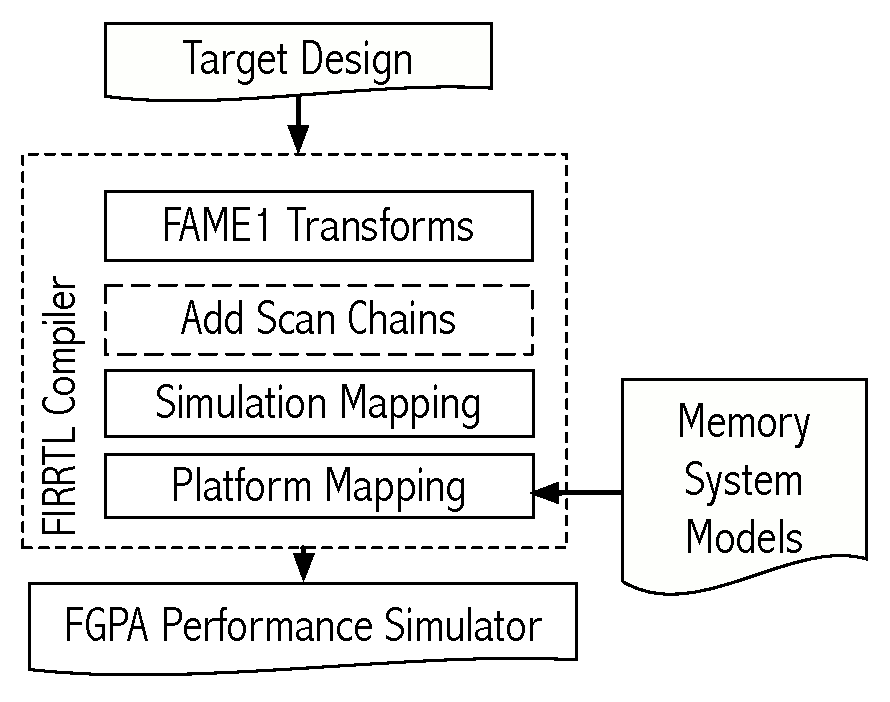
\includegraphics[width=7cm]{figures/firrtl.pdf}
	\caption{FIRRTL custom transforms for the FPGA simulator}
	\label{fig:firrtl}
\end{figure}

\section{Target Specification and Simulation Abstractions}

In MIDAS, the target design is specified as a synchronous dataflow network(SDF)
of \emph{models}, connected with FIFO \emph{channels}, that carry simulation
\emph{tokens}(messages), akin to the RAMP\cite{ramp} and APorts\cite{model}.
This abstraction is sufficient to captures the RTL behavior of the target,
while still enabling a wide range of optimizations that make FPGAs more
effective accelerators for simulation.

\emph{Models} model a single synchronous block of digital logic (an ALU, a
processor pipeline, a cache, etc...). A model \emph{fires} and advances one
cycle in target time, by dequeuing a single token from each of its input
channels, and has enqueuing a single token into each of its output channels
(updating local state if required).  Models must dequeue from each input, and
into enqueue each output exactly once before they may dequeue younger inputs;
they may never ``peek" at younger tokens.  Supposing, a model has no
side-effects, two implementations of a model are functionally indentical, if
for all sequences of input tokens I, and some intital state S0, they produce the
same sequence of output tokens O.

\emph{Tokens} are the basic quantum of data in the simulation. A token is
defined by a bitwidth, and a value, corresponding to the the bitwidth of the
wire that carries it, and value on that wire after it has settled for that
cycle(more on this later). Example: a 32-bit unit with a value of zero.

\emph{Channels} carry tokens between model in FIFO order, and model the
interconnect between those models. Channels may represent either a \emph{pipe}
(a wire with 0 or more registers) or a \emph{queue}(a latency-insenstive,
interface) in the target. Channels may also implement clock domain crossing
(CDC) by duplicating or dropping the tokens enqueued by the producer, based on
the relative clock frequency of the two models.\footnote{The channel differs
from a classical SDF channel in two ways. Firstly, to implement CDC in an SDF,
an intermediate process would need to be placed between two channels.  Second,
MIDAS channels are not infinitely deep. (Though, one could mimic a finite
channel in an SDF with a bidirectional pair of channels: one carrying the
original tokens from source to sink, and the second carrying credit tokens from
sink to source. This is effecively what happens in MIDAS, as models must check
there output queues are not full (equivalent to consuming a credit token)
before firing.)}

At time zero each of the channels is intialized with a sequence of tokens. In
MIDAS, this is defined by type of target interconnect they model.  A pipe is
intialized with tokens equal to it's latency (thus, a channel that models a
wire, is intialized with zero input tokens).

\emph{Deadlock} occurs if no model can advance (not all of its inputs are
valid, or it's outputs are not ready to accept a new token). Generally, this
occurs when the SDF includes a combinational path that passes through zero
or more other models before feeding back into itself. \TODO{This is
demonstrated in example K.} Judicious choice of target interconnect (using
latency insenstive channels, or pipes with non-zero latency) is required to
prevent this.

A simulation that faithfully implements an SDF of this form decouples
target-time from host-time: it may take an arbitrary (but finite) host-time for
tokens to pass through channels, or for models to fire.  Moreover, the
simulation may optimized automatically by performing transformations on models
that maintain their token input-output behavior.

When a model is hosted on an FPGA this implies that one target cycle may
execute over some number of FPGA clock cycles.  ASIC structures that map poorly
to an FPGA when implemented directly, like CAMs and multi-ported RAMs, can
instead by simulated over multiple FPGA cycles, with fewer resources and higher
FPGA clock frequency.


To help quantify this time-area trade off it is useful to define FPGA-cycle to Model-Cycle Ratio\cite{APorts}:
$$ FMR = \frac{Cycles_{FPGA}}{Cycles_{Target}} $$

\noindent The rate at which the model simulates is thus given by:

$$ f_{model} = \frac{f_{FPGA}}{FMR} $$

In principal, MIDAS can integrate any software or RTL model that obeys the semantics described above.


\section{The MIDAS Compiler Flow}


\subsection{Source Tranformations}

Source RTL must be transformed to conform to MIDAS' SDF model of computation.
To do this, MIDAS uses a FIRRTL compiler pass that adds an additional enable to
all target registers and sequential memories \TODO(See figure X). This baseline
model has an FMR of 1, assuming inputs are always available and its outputs
queues are never full.

Additional transformations may be invoked to add scan chains and I/O trace
buffers for debugging, and for state snapshotting for use with
Strober\cite{strober}.

\subsection{Simulation Mapping}

Once source RTL has been transformed into models, MIDAS generates host-agnostic
simulation-mapping of the SDF. Using Chisel3, MIDAS generates simulation queues
that implement the channels of the SDF. For source RTL, MIDAS ands the valids
of all of it's input channels, and the readies of all of its output channels to
targetFire input of the transformed module. If a channel would cross over the
boundary of the local FPGA, MIDAS generates an endpoint, a memory mapped queue,
whose sister endpoint on a different part of the host platform. Together, these
endpoints implement a channel.  MIDAS also emits widgets, that sequence the
automatically inserted scan chains, trace buffers, and a default I/O widget,
which ties off all I/O on models that were not explicitly connected in the SDF,
and a controller, that can reset simulation to time 0, and regulates the
advance of target time on the FPGA.

After simulation mapping, MIDAS has produced a module with a single AXI4 slave,
which will be used to configure the simulator, read instrumentation presented
by widgets, and read and write to simulation endpoints, and a AXI4 master,
which makes memory requests of the local FPGA memory system.


\subsection{Platform Mapping}

In attempt to orthogonalize MIDAS' from some of the complexities of FPGA
toolchains, MIDAS requires that each FPGA-host implements a skeleton project
that exposes standard interfaces to its periphery IP such as  memory
controllers for FPGA-local DRAM, and communication IP, like PCI-E and ethernet
controllers. Finally, these projects expose a clock and synchronous reset which
will drive the midas generated RTL.  During platform mapping, MIDAS bridges out
the AXI-4 master and slave interfaces to the interfaces presented by the
project.

Finally, MIDAS then emits a ``*Top.v" that can be compiled into the
aforementioned FPGA project, and a C++ header ``*consts.h" that describes the
memory map of simulator residing on that particular FPGA.

\section{MIDAS API \& Master Program}

To control the simulation, the user must compile a simulation master, linking
in the MIDAS C++ library, and the compiler generated header. This library
implement the primitive simulation commands of the MIDAS API, such as
\emph{step K}, \emph{reset}. Each of these commands is implemented with
simulation MMIO.  Widgets and models instantiated in in the simulator have
drivers that extend this API, again implemented simulation MMIO to their
hardware components. For example, the default I/O widget has \emph{peek} and
\emph{poke} to read and change the value of tied off signals.

At time of writing, the user is responsible for linking in their own software
models, and for moving tokens between endpoints (presently, implemented over
simulation MMIO).

\section{Target \& Host Machines of this Report}

While MIDAS has preliminary support for other host platforms, such as Catapult,
all the experiments of this report are run on Xilinx ZC706 development boards,
which feature a Zynq XC7Z045 FPGA. These FPGAs have a Processing System (PS),
consisting of hardened ARM A9 with 512 MiB of DRAM, connected to the
programmable logic(PL), which implements the Kintex-7 fabric architecture with
19.1Mb of BRAM and 350K logic cells. The PS is connected to the PL though a
number of interfaces, we use one of 32-bit AXI-4 ports. Linux processes
running on the PS interact with the PL with MMIO over this interface.  Finally,
the PL is connected to a configurable DDR PHY, which on the ZC706, drives a
DDR3 SODIMM (8GiB).

The target designs used throughout this report all have similar SDFs.
\TODO{Shown in figure X.} A single unit of RTL generated by RocketChip
including a single processor pipeline (Rocket or BOOM) with L1 caches, a
TileLink agent that manages a tether, by issuing TL requests tunneled over a
serial interface into the target's memory system. A software model wrapping the
RISC-V front-end server (FESVR) implements the host-side of the thether. The
FESVR is used to proxy console I/O to the host-machine.  Finally, a memory
timing model connects to rocketchip's an AXI4 slave interface, Remaining, I/O
coming off the transformed model, including reset, are bound to a default I/O
widget.

\begin{figure}
	\centering
	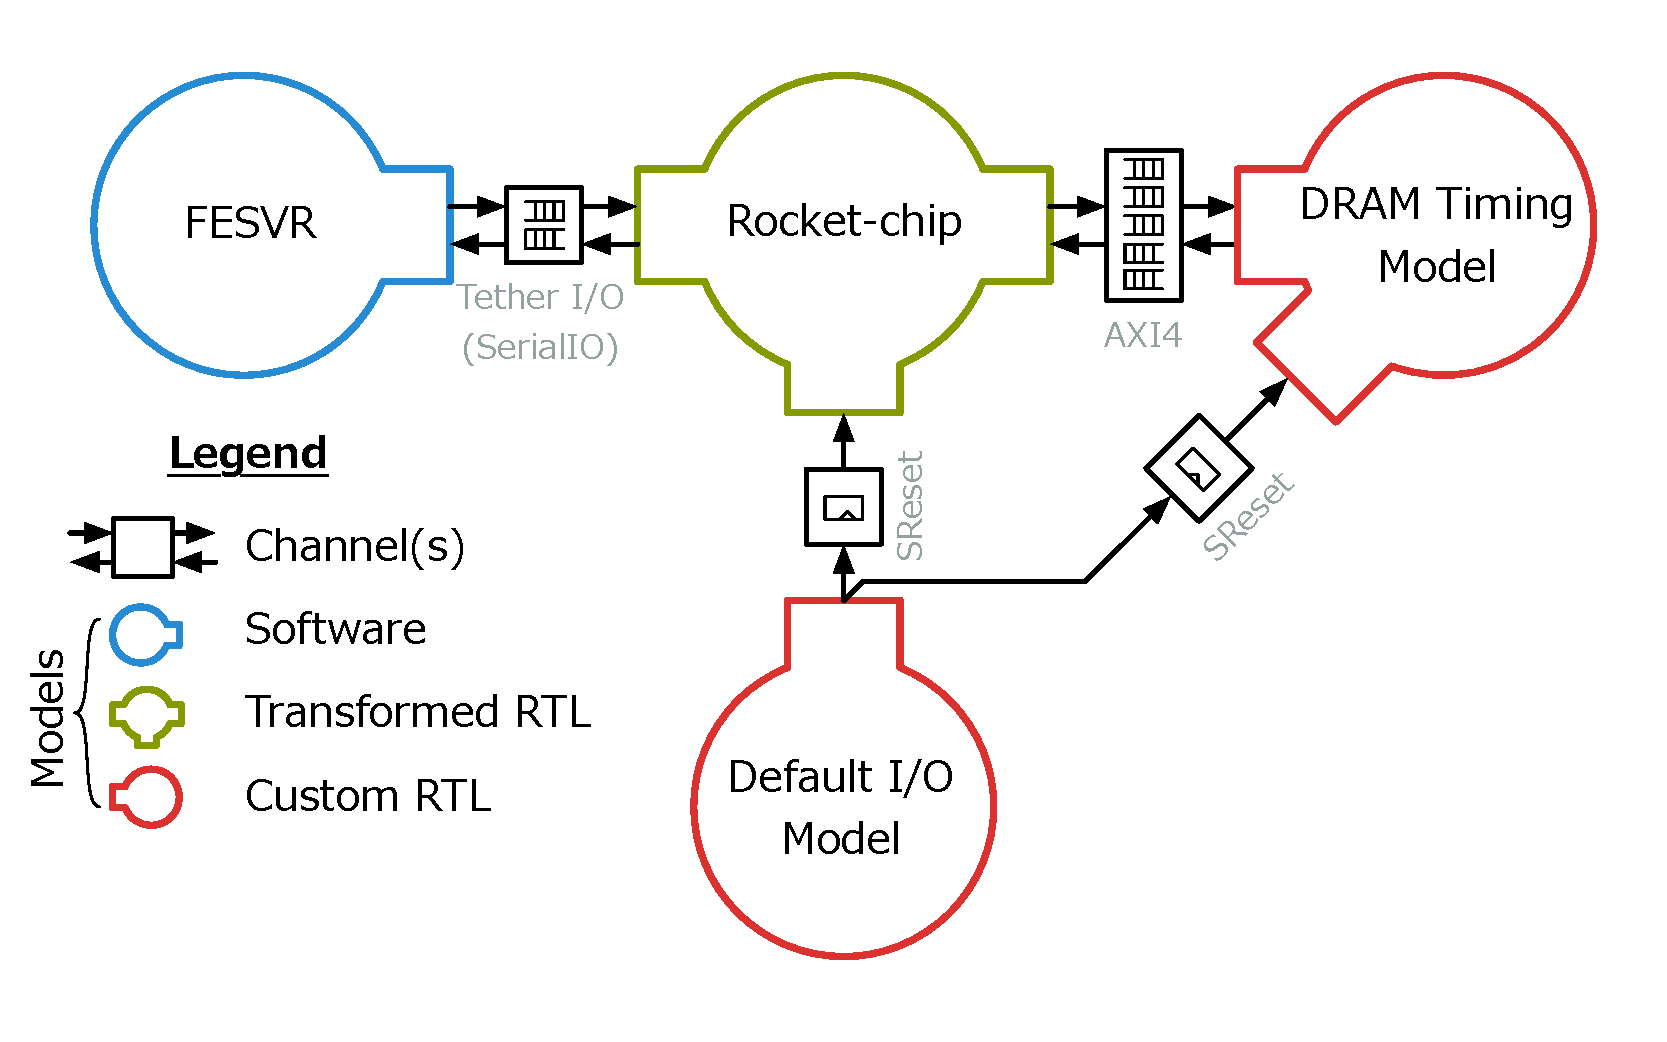
\includegraphics[width=16cm]{figures/masters-target.pdf}
    \caption{The MIDAS SDF of the target design used in this report. Channel
    details and initial tokens are omitted for simplicity. Both the Tether I/O
    and AXI4 have bidirectional decoupled (ready-valid) target interconnect,
    thus the channels model queues. SReset channels are pipes with
    a latency of one (a single register).}
	\label{fig:default-target}
\end{figure}

Thus unless stated otherwise, simulations are hosted with the master program
and FESVR model running on the PS, with the transformed RTL and memory-timing
model implemented in the PL. Simulation MMIO is mapped directly to reads and
writes over the AXI4 iterface exposed by the PS. Only the timing model and a
loadmem widget (used to intialize DRAM) make memory requests; these are issued
directly to the DDR3 controller of the PL.
